\documentclass{article}
\usepackage{amsmath}
\usepackage{amsfonts}
\usepackage{graphicx}
\graphicspath{{./images/}}
\usepackage{relsize}
\DeclareMathOperator*{\argmin}{argmin}
\DeclareMathOperator*{\argmax}{argmax}
\begin{document}
    
    \section{Task 15}
    Using the results produced on Task 9 we implement a Naive Bayes Classifier.
    This classifier is based on the assumption of independence between different features.
    In our example, where different features are actually different pixel colors the features themselves should be considered dependent.
    Therefore we expect the results of this classifier to be worse than those of a classifier that considers features to be dependent, such as sklearn's Gaussian Proccess Classifier.

    In comparison to the already implemented sklearn naive bayes classifier, our implementetation lacks the functionality of refiting new data incrementally.
    Specifically the corresponding sklearn classifier uses a function called partial fit, in order to refit the model faster, in case additional data are provided.
    
    Another interesting feature of the sklearn implementetation, which we decided to include as well, is the class attribute $\epsilon$.
    This attribute allows for the homogenization of the variances between different classes and features.
    It has been empirically shown that this smoothing process improves classifier perforamnce.
    
    In our specific case where the dataset contains images, a number of pixels of a digit are unaltered between different samples.
    In other words, some of the dataset's features have zero variance, leading to possible warnings of division by zero, during the prediction process.
    For this reason it is essential to introduce a smoothing parameter,in order to tackle this problem.

    We now present the accuracy score of our classifier for different values of $\epsilon$.
    Our models have been trained and tested on the same dataset. \newline
    After the optimal value for our hyperparameter is selected, we evaluate our model on the test set.
    Firstly, we use the same value as the sklearn classifier, in order to compare our results.
    The accuracy score for sklearn's implementation is $0.7587$.
    Subsequentlly we increase the factor as shown below:
    \begin{itemize}
        \item $\epsilon = 10 ^ {-9}$ Custom Naive Bayes score $= 0.7587$
        \item $\epsilon = 10 ^ {-7}$ Custom Naive Bayes score $= 0.7767$
        \item $\epsilon = 10 ^{-5}$ Custom Naive Bayes score $= 0.7907$
        \item $\epsilon = 10 ^ {-3}$ Custom Naive Bayes score $= 0.8132$
        \item $\epsilon = 10^{-1}$ Custom Naive Bayes score $= 0.8512$
    \end{itemize}

    To begin with, we observe that our classifier produces identical results with sklearn's classifier, when using the same $\epsilon$.
    Adiitionally, it is apparent that performance increases with $\epsilon$.
    Therefore for our model we select $\epsilon = 0.1$
    In general increasing $\epsilon$ might lead to overhomogenization, which in turn could hide substantial information from our model.
    In the next task we will observe in further detail the effects of overhomogenization on our model's performance.
    Speciffically, what happens to a model's accuracy when the variances of different features are falsely considered identical.

    Finally we evaluate our model's generalized score on the test set, for the selected hyperparameter.
    Custom Naive Bayes generalized score $= 0.8156$

    \section{Task 16}
    On the following task we repeat the process of classifying the test data and calculating the accuracy score.
    The difference here lies on the fact that we consider the variances of different features to be unitary.
    As said before, this is equivalent to completely homogenizing feauture variances.
    Therefore we expect the model fitted here, to have poorer perforamnce than the one fitted on task 15, as computed variances are indeed different.

    In this case of course, the hyperameter $\epsilon$ is redundant, as the variances are already identical.
    Therefore we just have to compute the accuracy score on the test set.
    Indeed we calculate the generalized score for the Naive Bayes classifier with unit var to be $0.8127$
    As we expected this model's score is lower than the previous ones' since the hypothesis of unitary variances is false.
    
    Interestingly enough, in the special case that class prior probabilities are equal,
    this model is equivalent to the EuclideanDistanceClassifier.

    \section{Task 18}
        \subsection{Part a}
    In this particular task we ideally want a metaclassifier that gives preference to a particular classifier, given his minimum misses.
    In other words our metaclassifier could 'pick' or give greater weight to the most trustworthy of predictions, given a matrix of minimum misses per classifier.
    Having said the above we present a matrix with the number of wrongly classified samples for every digit and classifier.

    \begin{figure}[ht]
        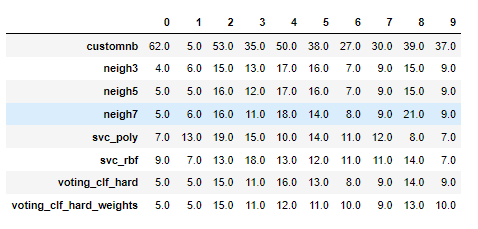
\includegraphics[width = 1.1\textwidth]{Classifiers_mistakes}
    \end{figure}
    \newpage
    Scanning this matrix it is easy to find the minimum misses for each digit:

        \begin{table}[ht]
            \centering
        
            \begin{tabular}{|c| c| c|}
            \hline
            class & minimum missed & optimal classifier \\
            \hline
            0 & 4 & knn(3)\\
            1 & 5 & knn(5) \\
            2 & 13 & svc(rbf) \\
            3 & 11 & knn(7) \\
            4 & 10 & svc(poly) \\
            5 & 12 & svc(rbf) \\
            6 & 7 & knn(5) \\
            7 & 9 & knn(5) \\
            8 & 8 & svc(poly) \\
            9 & 7 & svc(poly) \\
            \hline
            \end{tabular}
        \end{table}
    
    So, our theoretical metaclassifier should have an accuracy score given by the following formula:
    \[Accuracy = \frac{TotalSamples - \sum\limits_{class =0}^{9}MinimumMisses(class)}{TotalSamples}\]
    Which in our case equals to 0.957. This number can be used as an empirical upper bound for the implemented model.

    In practice though, our model will be selected by finding complementary mistakes between individual classifiers.
    Specifically we will aggregate all tuples of classifiers with different minimum of digit scores.
    For example on the table shown above, the classifier NearestNeighbors(3) has a minimum of digit scores at digit 4, while the classifier SupportVectorMachine(poly) has a minimum at digit 2,
    making them potential members of a tuple.
    This way the worst mistakes made by one classifier can be corrected by the others during the voting process.
    In order to avoid stalemates the number of classifiers selected must be odd.

    Finally after all potential tuples are aggregated, we select the one with the maximum accuracy score computed on the training data set.
    The base models used in our search derive from the best models, evaluated during task 17.
    Specifically we select among all available svc models (based on the different kernel and gamma parameters), Gaussian Naive Bayes and KNearestNeighbors with k between 3 and 7.
    The model selected will be further weighted to check for performance differences.
    The Voting Classifier that emerges from the above search is:
    \newpage

    \begin{table}[ht]
        \centering
        \begin{tabular}{| c | c |}
            \hline
            \multicolumn{2}{|c|}{BestVotingClassifier}\\
            \hline
            \rule{0pt}{4ex} \large Classifier Name & \large Classifier Parameters\\
            \hline
            KNearestNeighbors & number of neighbors = 4 \\ \hline
            SupportVectorMachine & kernel = polynomial \\ \hline
            SupportVectorMachine & kernel = linear \\ \hline
            SupportVectorMachine & kernel = rbf \\ \hline
            GaussianNaiveBayes  &  parameters = default \\ \hline
        \end{tabular}
    \end{table}
    In order to fit the svcs, the data have firstly been scaled properly.
    After the model has been selected we experiment with different weights to each base classifier, with no significant difference on its perforamnce.
    The model's score on the test data is finally being calulated.\\ 
    Generalized score of the best VotingClassifier = 0.9487


\subsection{Part b}
In this task we are implementing a baggingclassifier based on the models trained during task 17.
For this meta-classifier a single base classifier is selected and trained repeatedly on different subsets of features and samples from our train dataset, using bootstarp aggregation. 

This technique, draws a predefined number of samples and features randomly for each model and uses that set to train it. 
In our case we have used bootstrap only for our samples, as bagging for features was not expected to  produced significant performance increases.

Our implementation relies solely on the classifier found using gridsearch, as this model had the best score.
We remind that the model given by grisearch was an SVC with $C = 10, \gamma = 5* 10^ {-3}$. Before fitting our model we have scaled our train data.
We experiment with different numbers of samples and features for each classifier.
Below are the training scores of our model for the different parameters:
\begin{table}[ht]
    
    \begin{tabular}{| c | c | c |}  
        
        \hline
        \rule{0pt}{4ex} \large Number of samples(\%) & \large Number of features(\%) & \large Accuracy Score \\
        \hline
        0.1 & 0.1 & 0.88424 \\
        \hline
        0.1 & 0.55 & 0.9147\\
        \hline
        0.1 & 1.0 & 0.9220 \\
        \hline        
        0.55 & 0.1 & 0.9494\\
        \hline
        0.55 & 0.55 & 0.9728 \\
        \hline
        0.55 & 1.0 & 0.9770\\
        \hline
        1.0 & 0.1 & 0.9557 \\
        \hline
        1.0 & 0.55 & 0.9768 \\
        \hline
        1.0 & 1.0 & 0.9792 \\
        \hline 
    \end{tabular}
\end{table}
\newpage
We observe that accuracy increases with the percentage of features.
Given that our features represent pixel colors of a digit, naturally we require a large percentage of features to make a proper prediction.
Finally we calculate our generalized score on the baggingclassifier with parameters\\
\((number \ of \ samples, number \ of \ features) = (1.0, 1.0)\).\\
Generalized score for baggingclassifier $=0.9506$



\end{document}

